\documentclass[twoside]{book}

% Packages required by doxygen
\usepackage{fixltx2e}
\usepackage{calc}
\usepackage{doxygen}
\usepackage[export]{adjustbox} % also loads graphicx
\usepackage{graphicx}
\usepackage[utf8]{inputenc}
\usepackage{makeidx}
\usepackage{multicol}
\usepackage{multirow}
\PassOptionsToPackage{warn}{textcomp}
\usepackage{textcomp}
\usepackage[nointegrals]{wasysym}
\usepackage[table]{xcolor}

% Font selection
\usepackage[T1]{fontenc}
\usepackage[scaled=.90]{helvet}
\usepackage{courier}
\usepackage{amssymb}
\usepackage{sectsty}
\renewcommand{\familydefault}{\sfdefault}
\allsectionsfont{%
  \fontseries{bc}\selectfont%
  \color{darkgray}%
}
\renewcommand{\DoxyLabelFont}{%
  \fontseries{bc}\selectfont%
  \color{darkgray}%
}
\newcommand{\+}{\discretionary{\mbox{\scriptsize$\hookleftarrow$}}{}{}}

% Page & text layout
\usepackage{geometry}
\geometry{%
  a4paper,%
  top=2.5cm,%
  bottom=2.5cm,%
  left=2.5cm,%
  right=2.5cm%
}
\tolerance=750
\hfuzz=15pt
\hbadness=750
\setlength{\emergencystretch}{15pt}
\setlength{\parindent}{0cm}
\setlength{\parskip}{3ex plus 2ex minus 2ex}
\makeatletter
\renewcommand{\paragraph}{%
  \@startsection{paragraph}{4}{0ex}{-1.0ex}{1.0ex}{%
    \normalfont\normalsize\bfseries\SS@parafont%
  }%
}
\renewcommand{\subparagraph}{%
  \@startsection{subparagraph}{5}{0ex}{-1.0ex}{1.0ex}{%
    \normalfont\normalsize\bfseries\SS@subparafont%
  }%
}
\makeatother

% Headers & footers
\usepackage{fancyhdr}
\pagestyle{fancyplain}
\fancyhead[LE]{\fancyplain{}{\bfseries\thepage}}
\fancyhead[CE]{\fancyplain{}{}}
\fancyhead[RE]{\fancyplain{}{\bfseries\leftmark}}
\fancyhead[LO]{\fancyplain{}{\bfseries\rightmark}}
\fancyhead[CO]{\fancyplain{}{}}
\fancyhead[RO]{\fancyplain{}{\bfseries\thepage}}
\fancyfoot[LE]{\fancyplain{}{}}
\fancyfoot[CE]{\fancyplain{}{}}
\fancyfoot[RE]{\fancyplain{}{\bfseries\scriptsize Generated by Doxygen }}
\fancyfoot[LO]{\fancyplain{}{\bfseries\scriptsize Generated by Doxygen }}
\fancyfoot[CO]{\fancyplain{}{}}
\fancyfoot[RO]{\fancyplain{}{}}
\renewcommand{\footrulewidth}{0.4pt}
\renewcommand{\chaptermark}[1]{%
  \markboth{#1}{}%
}
\renewcommand{\sectionmark}[1]{%
  \markright{\thesection\ #1}%
}

% Indices & bibliography
\usepackage{natbib}
\usepackage[titles]{tocloft}
\setcounter{tocdepth}{3}
\setcounter{secnumdepth}{5}
\makeindex

% Hyperlinks (required, but should be loaded last)
\usepackage{ifpdf}
\ifpdf
  \usepackage[pdftex,pagebackref=true]{hyperref}
\else
  \usepackage[ps2pdf,pagebackref=true]{hyperref}
\fi
\hypersetup{%
  colorlinks=true,%
  linkcolor=blue,%
  citecolor=blue,%
  unicode%
}

% Custom commands
\newcommand{\clearemptydoublepage}{%
  \newpage{\pagestyle{empty}\cleardoublepage}%
}

\usepackage{caption}
\captionsetup{labelsep=space,justification=centering,font={bf},singlelinecheck=off,skip=4pt,position=top}

%===== C O N T E N T S =====

\begin{document}

% Titlepage & ToC
\hypersetup{pageanchor=false,
             bookmarksnumbered=true,
             pdfencoding=unicode
            }
\pagenumbering{alph}
\begin{titlepage}
\vspace*{7cm}
\begin{center}%
{\Large My Project }\\
\vspace*{1cm}
{\large Generated by Doxygen 1.8.14}\\
\end{center}
\end{titlepage}
\clearemptydoublepage
\pagenumbering{roman}
\tableofcontents
\clearemptydoublepage
\pagenumbering{arabic}
\hypersetup{pageanchor=true}

%--- Begin generated contents ---
\chapter{Namespace Index}
\section{Namespace List}
Here is a list of all documented namespaces with brief descriptions\+:\begin{DoxyCompactList}
\item\contentsline{section}{\mbox{\hyperlink{namespace_hannes_o_o_p_project}{Hannes\+O\+O\+P\+Project}} \\*Description of this project }{\pageref{namespace_hannes_o_o_p_project}}{}
\end{DoxyCompactList}

\chapter{Hierarchical Index}
\section{Class Hierarchy}
This inheritance list is sorted roughly, but not completely, alphabetically\+:\begin{DoxyCompactList}
\item \contentsline{section}{O\+O\+P.\+Analysis}{\pageref{class_o_o_p_1_1_analysis}}{}
\item \contentsline{section}{O\+O\+P\+\_\+np\+Array.\+Analysis}{\pageref{class_o_o_p__np_array_1_1_analysis}}{}
\item \contentsline{section}{O\+O\+P\+\_\+np\+Array.\+Builder}{\pageref{class_o_o_p__np_array_1_1_builder}}{}
\item \contentsline{section}{O\+O\+P.\+Builder}{\pageref{class_o_o_p_1_1_builder}}{}
\item \contentsline{section}{O\+O\+P\+\_\+np\+Array.\+Cytokine}{\pageref{class_o_o_p__np_array_1_1_cytokine}}{}
\item \contentsline{section}{O\+O\+P.\+Cytokine}{\pageref{class_o_o_p_1_1_cytokine}}{}
\item \contentsline{section}{O\+O\+P.\+Glycan}{\pageref{class_o_o_p_1_1_glycan}}{}
\item \contentsline{section}{O\+O\+P\+\_\+np\+Array.\+Glycan}{\pageref{class_o_o_p__np_array_1_1_glycan}}{}
\item \contentsline{section}{O\+O\+P.\+Lectin}{\pageref{class_o_o_p_1_1_lectin}}{}
\item \contentsline{section}{O\+O\+P\+\_\+np\+Array.\+Lectin}{\pageref{class_o_o_p__np_array_1_1_lectin}}{}
\item \contentsline{section}{O\+O\+P.\+Simulation}{\pageref{class_o_o_p_1_1_simulation}}{}
\item \contentsline{section}{O\+O\+P\+\_\+np\+Array.\+Simulation}{\pageref{class_o_o_p__np_array_1_1_simulation}}{}
\item \contentsline{section}{O\+O\+P.\+Sphere}{\pageref{class_o_o_p_1_1_sphere}}{}
\begin{DoxyCompactList}
\item \contentsline{section}{O\+O\+P.\+Bead}{\pageref{class_o_o_p_1_1_bead}}{}
\item \contentsline{section}{O\+O\+P.\+Decoder\+Cell}{\pageref{class_o_o_p_1_1_decoder_cell}}{}
\end{DoxyCompactList}
\item \contentsline{section}{O\+O\+P\+\_\+np\+Array.\+Sphere}{\pageref{class_o_o_p__np_array_1_1_sphere}}{}
\begin{DoxyCompactList}
\item \contentsline{section}{O\+O\+P\+\_\+np\+Array.\+Bead}{\pageref{class_o_o_p__np_array_1_1_bead}}{}
\item \contentsline{section}{O\+O\+P\+\_\+np\+Array.\+Decoder\+Cell}{\pageref{class_o_o_p__np_array_1_1_decoder_cell}}{}
\end{DoxyCompactList}
\item \contentsline{section}{O\+O\+P\+\_\+np\+Array.\+Well}{\pageref{class_o_o_p__np_array_1_1_well}}{}
\begin{DoxyCompactList}
\item \contentsline{section}{O\+O\+P\+\_\+np\+Array.\+Well\+\_\+list}{\pageref{class_o_o_p__np_array_1_1_well__list}}{}
\item \contentsline{section}{O\+O\+P\+\_\+np\+Array.\+Well\+\_\+np\+Array}{\pageref{class_o_o_p__np_array_1_1_well__np_array}}{}
\end{DoxyCompactList}
\item \contentsline{section}{O\+O\+P.\+Well}{\pageref{class_o_o_p_1_1_well}}{}
\end{DoxyCompactList}

\chapter{Class Index}
\section{Class List}
Here are the classes, structs, unions and interfaces with brief descriptions\+:\begin{DoxyCompactList}
\item\contentsline{section}{\mbox{\hyperlink{class_o_o_p_1_1_cell}{O\+O\+P.\+Cell}} \\*Dokumentation for class \mbox{\hyperlink{class_o_o_p_1_1_cell}{Cell}} }{\pageref{class_o_o_p_1_1_cell}}{}
\item\contentsline{section}{\mbox{\hyperlink{class_o_o_p_1_1_decoder_cell}{O\+O\+P.\+Decoder\+Cell}} }{\pageref{class_o_o_p_1_1_decoder_cell}}{}
\item\contentsline{section}{\mbox{\hyperlink{class_o_o_p_1_1_encoder_cell}{O\+O\+P.\+Encoder\+Cell}} }{\pageref{class_o_o_p_1_1_encoder_cell}}{}
\item\contentsline{section}{\mbox{\hyperlink{class_o_o_p_1_1_glycan}{O\+O\+P.\+Glycan}} }{\pageref{class_o_o_p_1_1_glycan}}{}
\item\contentsline{section}{\mbox{\hyperlink{class_o_o_p_1_1_lectin}{O\+O\+P.\+Lectin}} }{\pageref{class_o_o_p_1_1_lectin}}{}
\item\contentsline{section}{\mbox{\hyperlink{classprototype_1_1_object_factory}{prototype.\+Object\+Factory}} }{\pageref{classprototype_1_1_object_factory}}{}
\item\contentsline{section}{\mbox{\hyperlink{classprototype_1_1_prototype}{prototype.\+Prototype}} }{\pageref{classprototype_1_1_prototype}}{}
\item\contentsline{section}{\mbox{\hyperlink{classprototype_1_1_type1}{prototype.\+Type1}} }{\pageref{classprototype_1_1_type1}}{}
\item\contentsline{section}{\mbox{\hyperlink{classprototype_1_1_type2}{prototype.\+Type2}} }{\pageref{classprototype_1_1_type2}}{}
\end{DoxyCompactList}

\chapter{Namespace Documentation}
\hypertarget{namespace_cytokines}{}\section{Cytokines Namespace Reference}
\label{namespace_cytokines}\index{Cytokines@{Cytokines}}


Hannes Baukmann\textquotesingle{}s Course Completion Project.  




\subsection{Detailed Description}
Hannes Baukmann\textquotesingle{}s Course Completion Project. 

This project aims to simulate the binding of immune cells to artificial beads decorated with molecules that induce a biological response of the cells. In nature, immene cells express receptors (so-\/called lectins) binding to carbohydrate structures, or glycans, on the surface of body\textquotesingle{}s own cells or pathogens. Depending on the nature of the glycan ligand, cells express specific cytokines, e. g. the pro-\/inflammatory I\+L-\/6. The idea of the biochemical is to investigate the biological response of a monocytic cell line which recombinantly expresses a defined set of lectin receptors upon binding to glycan ligands that are chemically linked to acrylic glass beads in well-\/defined amounts.

In the following, the translation of real-\/world dimensions for this project will be explained.

Monocytes are 5--20 um in diameter, while beads typically are few um in size. By definition, 1 pt in this program corresponds to 10 um in reality. The (round) basis of a well used in these experiments has an area of 0.\+36 qcm. Here, we consider a quadratic basis, hence $x=y=0.06 cm=600 pt$. Typical volume is 25 ul. Hence, the height of the liquid in a well is \[ h = \frac{25 \mu l}{b} = \frac{25 \cdot 10^{-8} m^3}{0.36 cm^2} = 41.67 \cdot 10^{-4} m = 420 pt. \] The number of cells usually used in these experiments is 50,000, incubated with a five-\/fold excess of beads. To make calculations feasible, the well dimension are reduced ten-\/fold in every dimension. In order to maintain equal density of particles, the number of cells and beads are consequently reduced to 50 and 250, respectively.

The incubation time of the cells with beads amounts to 30 minutes, or 1800 s. In order to determine to many steps that correlates to, the Stokes-\/\+Einstein equation was utilized\+: \[ x^2 = \frac{k_B \cdot T}{6r \pi \eta} t = \frac{1.381 \cdot 10^{-23} J/K \cdot 298 K}{6 \cdot 5 \mu m \cdot \pi \cdot 0.891 mPa \cdot s} = 9.8 \cdot 10^{-13} \frac{m^2}{s} \cdot t \] At 1 s, a particle of 10 um in aqueous solution would diffuse (ignoring the influence of gravity on sinking particles)\+: \[ \sqrt{x^2} = \sqrt{4.9 \cdot 10^{-13} \frac{m^2}{s} \cdot 1s} = 7 \cdot 10^{-7} m.\] Therefore, a typical experiment of 30 minutes corresponds to $ 1800 s \cdot 0.7 \mu m/s = 1260 \mu m = 126\mbox{ steps}. $

In summary, the values used are\+: \tabulinesep=1mm
\begin{longtabu} spread 0pt [c]{*{4}{|X[-1]}|}
\hline
\rowcolor{\tableheadbgcolor}\textbf{ Parameter  }&\textbf{ Value ({\itshape in vitro})  }&\textbf{ Value ({\itshape in silico})  }&\textbf{ Reduced value   }\\\cline{1-4}
\endfirsthead
\hline
\endfoot
\hline
\rowcolor{\tableheadbgcolor}\textbf{ Parameter  }&\textbf{ Value ({\itshape in vitro})  }&\textbf{ Value ({\itshape in silico})  }&\textbf{ Reduced value   }\\\cline{1-4}
\endhead
Cell size  &5-\/20 um  &1 pt  &---   \\\cline{1-4}
Bead size  &few um  &1 pt  &---   \\\cline{1-4}
Well basis  &0.\+36 qcm  &600 pt $\ast$ 600 pt  &60 pt, 60 pt   \\\cline{1-4}
Volume  &25 ul  &basis $\ast$ 420 pt  &42 pt   \\\cline{1-4}
Number of cells  &50,000  &50,000  &50   \\\cline{1-4}
Number of beads  &250,000  &250,000  &250   \\\cline{1-4}
Incubation time  &30 min  &126 steps  &---   \\\cline{1-4}
\end{longtabu}


The pairs of lectins, glycans, and cytokines implemented in the dictionary (vide infra) now (Aug 31, 2018) are\+:

\tabulinesep=1mm
\begin{longtabu} spread 0pt [c]{*{5}{|X[-1]}|}
\hline
\rowcolor{\tableheadbgcolor}\textbf{ Lectin  }&\textbf{ Glycan  }&\textbf{ Glycan type  }&\textbf{ Cytokine  }&\textbf{ Reference   }\\\cline{1-5}
\endfirsthead
\hline
\endfoot
\hline
\rowcolor{\tableheadbgcolor}\textbf{ Lectin  }&\textbf{ Glycan  }&\textbf{ Glycan type  }&\textbf{ Cytokine  }&\textbf{ Reference   }\\\cline{1-5}
\endhead
D\+C-\/\+S\+I\+GN  &Mannan  &Mannose  &I\+L-\/6  &1   \\\cline{1-5}
D\+C-\/\+S\+I\+GN  &Lewis-\/Y  &Fucose  &I\+L-\/27p28  &1   \\\cline{1-5}
Dectin-\/1  &Mannan  &Mannose  &I\+L-\/6  &1   \\\cline{1-5}
\end{longtabu}
1) Geijtenbeek, T. B. H. and Gringhuis, S. I. (2016) C-\/type lectin receptors in the control of T helper cell differentiation. {\itshape Nat Rev Immunol} 16(7)\+:433. 
\chapter{Class Documentation}
\hypertarget{class_c_c_p___hannes_1_1_analysis}{}\section{C\+C\+P\+\_\+\+Hannes.\+Analysis Class Reference}
\label{class_c_c_p___hannes_1_1_analysis}\index{C\+C\+P\+\_\+\+Hannes.\+Analysis@{C\+C\+P\+\_\+\+Hannes.\+Analysis}}


This class contains three methods for the analysis of the results from the \mbox{\hyperlink{class_c_c_p___hannes_1_1_simulation}{Simulation}}.  


\subsection*{Public Member Functions}
\begin{DoxyCompactItemize}
\item 
\mbox{\Hypertarget{class_c_c_p___hannes_1_1_analysis_a05c37e0523e8c7de03b8b808d1db1ae0}\label{class_c_c_p___hannes_1_1_analysis_a05c37e0523e8c7de03b8b808d1db1ae0}} 
def {\bfseries \+\_\+\+\_\+init\+\_\+\+\_\+} (self, simulation\+Results, cytokine\+\_\+names=None)
\item 
def \mbox{\hyperlink{class_c_c_p___hannes_1_1_analysis_a914957b746c4d5d7b13daa2786cc4ae6}{count\+Cytokines}} (self)
\begin{DoxyCompactList}\small\item\em Counts number of objects of class \mbox{\hyperlink{class_c_c_p___hannes_1_1_cytokine}{Cytokine}} of respective type, i. \end{DoxyCompactList}\item 
def \mbox{\hyperlink{class_c_c_p___hannes_1_1_analysis_aa008afd3924050a0634ffdde72b3e9d9}{plot\+Cytokines}} (self)
\begin{DoxyCompactList}\small\item\em Creates a bar graph of the numbers of each type of cytokine. \end{DoxyCompactList}\item 
def \mbox{\hyperlink{class_c_c_p___hannes_1_1_analysis_a4802fb98580b33a45025d96b64f21358}{plot\+Coordinates}} (self)
\begin{DoxyCompactList}\small\item\em Creates a 3D scatter plot of the coordinates where a \mbox{\hyperlink{class_c_c_p___hannes_1_1_bead}{Bead}} and a \mbox{\hyperlink{class_c_c_p___hannes_1_1_decoder_cell}{Decoder\+Cell}} met and produced a \mbox{\hyperlink{class_c_c_p___hannes_1_1_cytokine}{Cytokine}}. \end{DoxyCompactList}\end{DoxyCompactItemize}
\subsection*{Public Attributes}
\begin{DoxyCompactItemize}
\item 
\mbox{\Hypertarget{class_c_c_p___hannes_1_1_analysis_a4cea02ae53dd6b2bc1f51af6019851fc}\label{class_c_c_p___hannes_1_1_analysis_a4cea02ae53dd6b2bc1f51af6019851fc}} 
{\bfseries results}
\item 
\mbox{\Hypertarget{class_c_c_p___hannes_1_1_analysis_abbbe87ef8fd97908041d6af5cef9485d}\label{class_c_c_p___hannes_1_1_analysis_abbbe87ef8fd97908041d6af5cef9485d}} 
{\bfseries cytokine\+Names}
\item 
\mbox{\Hypertarget{class_c_c_p___hannes_1_1_analysis_a3f3659415fcff5636549a12bf7560930}\label{class_c_c_p___hannes_1_1_analysis_a3f3659415fcff5636549a12bf7560930}} 
{\bfseries cytokine\+Amount}
\end{DoxyCompactItemize}


\subsection{Detailed Description}
This class contains three methods for the analysis of the results from the \mbox{\hyperlink{class_c_c_p___hannes_1_1_simulation}{Simulation}}. 


\begin{DoxyParams}[1]{Parameters}
\mbox{\tt in}  & {\em simulation\+Results} & The results of the simulation, i. e. the list containing the \mbox{\hyperlink{class_c_c_p___hannes_1_1_cytokine}{Cytokine}} object produced. \\
\hline
\mbox{\tt in}  & {\em cytokine\+\_\+names} & Names of the cytokines to be analyzed (optional) \\
\hline
\end{DoxyParams}


\subsection{Member Function Documentation}
\mbox{\Hypertarget{class_c_c_p___hannes_1_1_analysis_a914957b746c4d5d7b13daa2786cc4ae6}\label{class_c_c_p___hannes_1_1_analysis_a914957b746c4d5d7b13daa2786cc4ae6}} 
\index{C\+C\+P\+\_\+\+Hannes\+::\+Analysis@{C\+C\+P\+\_\+\+Hannes\+::\+Analysis}!count\+Cytokines@{count\+Cytokines}}
\index{count\+Cytokines@{count\+Cytokines}!C\+C\+P\+\_\+\+Hannes\+::\+Analysis@{C\+C\+P\+\_\+\+Hannes\+::\+Analysis}}
\subsubsection{\texorpdfstring{count\+Cytokines()}{countCytokines()}}
{\footnotesize\ttfamily def C\+C\+P\+\_\+\+Hannes.\+Analysis.\+count\+Cytokines (\begin{DoxyParamCaption}\item[{}]{self }\end{DoxyParamCaption})}



Counts number of objects of class \mbox{\hyperlink{class_c_c_p___hannes_1_1_cytokine}{Cytokine}} of respective type, i. 

e. amount of cytokines produced.


\begin{DoxyParams}[1]{Parameters}
\mbox{\tt out}  & {\em self.\+cytokine\+Names} & List with name of cytokines. \\
\hline
\mbox{\tt out}  & {\em self.\+cytokine\+Amount} & List with amount of respective cytokine. \\
\hline
\end{DoxyParams}
\mbox{\Hypertarget{class_c_c_p___hannes_1_1_analysis_a4802fb98580b33a45025d96b64f21358}\label{class_c_c_p___hannes_1_1_analysis_a4802fb98580b33a45025d96b64f21358}} 
\index{C\+C\+P\+\_\+\+Hannes\+::\+Analysis@{C\+C\+P\+\_\+\+Hannes\+::\+Analysis}!plot\+Coordinates@{plot\+Coordinates}}
\index{plot\+Coordinates@{plot\+Coordinates}!C\+C\+P\+\_\+\+Hannes\+::\+Analysis@{C\+C\+P\+\_\+\+Hannes\+::\+Analysis}}
\subsubsection{\texorpdfstring{plot\+Coordinates()}{plotCoordinates()}}
{\footnotesize\ttfamily def C\+C\+P\+\_\+\+Hannes.\+Analysis.\+plot\+Coordinates (\begin{DoxyParamCaption}\item[{}]{self }\end{DoxyParamCaption})}



Creates a 3D scatter plot of the coordinates where a \mbox{\hyperlink{class_c_c_p___hannes_1_1_bead}{Bead}} and a \mbox{\hyperlink{class_c_c_p___hannes_1_1_decoder_cell}{Decoder\+Cell}} met and produced a \mbox{\hyperlink{class_c_c_p___hannes_1_1_cytokine}{Cytokine}}. 

\mbox{\Hypertarget{class_c_c_p___hannes_1_1_analysis_aa008afd3924050a0634ffdde72b3e9d9}\label{class_c_c_p___hannes_1_1_analysis_aa008afd3924050a0634ffdde72b3e9d9}} 
\index{C\+C\+P\+\_\+\+Hannes\+::\+Analysis@{C\+C\+P\+\_\+\+Hannes\+::\+Analysis}!plot\+Cytokines@{plot\+Cytokines}}
\index{plot\+Cytokines@{plot\+Cytokines}!C\+C\+P\+\_\+\+Hannes\+::\+Analysis@{C\+C\+P\+\_\+\+Hannes\+::\+Analysis}}
\subsubsection{\texorpdfstring{plot\+Cytokines()}{plotCytokines()}}
{\footnotesize\ttfamily def C\+C\+P\+\_\+\+Hannes.\+Analysis.\+plot\+Cytokines (\begin{DoxyParamCaption}\item[{}]{self }\end{DoxyParamCaption})}



Creates a bar graph of the numbers of each type of cytokine. 



The documentation for this class was generated from the following file\+:\begin{DoxyCompactItemize}
\item 
C\+C\+P\+\_\+\+Hannes.\+py\end{DoxyCompactItemize}

\hypertarget{class_c_c_p___hannes_1_1_bead}{}\section{C\+C\+P\+\_\+\+Hannes.\+Bead Class Reference}
\label{class_c_c_p___hannes_1_1_bead}\index{C\+C\+P\+\_\+\+Hannes.\+Bead@{C\+C\+P\+\_\+\+Hannes.\+Bead}}


\mbox{\hyperlink{class_c_c_p___hannes_1_1_bead}{Bead}} is a subclass of \mbox{\hyperlink{class_c_c_p___hannes_1_1_sphere}{Sphere}} and represents beads (made of acrylic glass) loaded with glycan structures.  


Inheritance diagram for C\+C\+P\+\_\+\+Hannes.\+Bead\+:\begin{figure}[H]
\begin{center}
\leavevmode
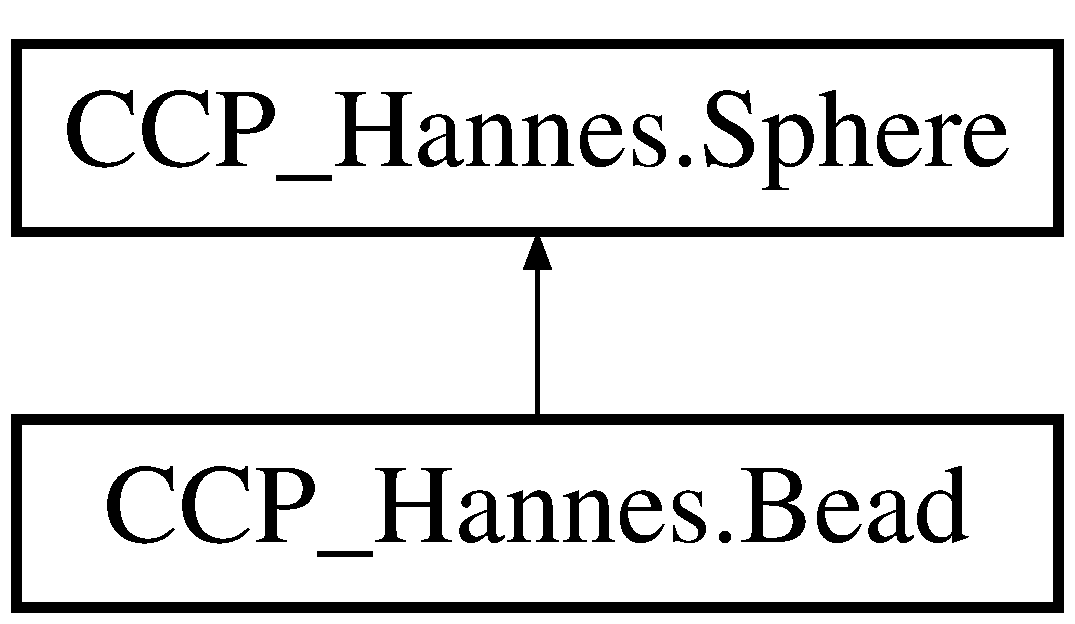
\includegraphics[height=2.000000cm]{class_c_c_p___hannes_1_1_bead}
\end{center}
\end{figure}
\subsection*{Public Member Functions}
\begin{DoxyCompactItemize}
\item 
\mbox{\Hypertarget{class_c_c_p___hannes_1_1_bead_a240f28f06e51c26dbd73255b1871bfa7}\label{class_c_c_p___hannes_1_1_bead_a240f28f06e51c26dbd73255b1871bfa7}} 
def {\bfseries \+\_\+\+\_\+init\+\_\+\+\_\+} (self, args)
\item 
def \mbox{\hyperlink{class_c_c_p___hannes_1_1_bead_a0da1639096e0bdd18ef542a01b2dab0f}{attach\+Glycans}} (self, glycan\+\_\+names\+\_\+list, glycan\+\_\+types\+\_\+list, density\+\_\+percentage)
\begin{DoxyCompactList}\small\item\em Method to attach \mbox{\hyperlink{class_c_c_p___hannes_1_1_glycan}{Glycan}} objects to \mbox{\hyperlink{class_c_c_p___hannes_1_1_bead}{Bead}} objects. \end{DoxyCompactList}\end{DoxyCompactItemize}
\subsection*{Public Attributes}
\begin{DoxyCompactItemize}
\item 
\mbox{\Hypertarget{class_c_c_p___hannes_1_1_bead_aab2ee2d3ff67f268fbee3c3d53b6e24d}\label{class_c_c_p___hannes_1_1_bead_aab2ee2d3ff67f268fbee3c3d53b6e24d}} 
{\bfseries glycan\+\_\+density}
\item 
\mbox{\Hypertarget{class_c_c_p___hannes_1_1_bead_a36e304460dd84f029c201d13a56cb590}\label{class_c_c_p___hannes_1_1_bead_a36e304460dd84f029c201d13a56cb590}} 
{\bfseries glycan}
\end{DoxyCompactItemize}


\subsection{Detailed Description}
\mbox{\hyperlink{class_c_c_p___hannes_1_1_bead}{Bead}} is a subclass of \mbox{\hyperlink{class_c_c_p___hannes_1_1_sphere}{Sphere}} and represents beads (made of acrylic glass) loaded with glycan structures. 

\subsection{Member Function Documentation}
\mbox{\Hypertarget{class_c_c_p___hannes_1_1_bead_a0da1639096e0bdd18ef542a01b2dab0f}\label{class_c_c_p___hannes_1_1_bead_a0da1639096e0bdd18ef542a01b2dab0f}} 
\index{C\+C\+P\+\_\+\+Hannes\+::\+Bead@{C\+C\+P\+\_\+\+Hannes\+::\+Bead}!attach\+Glycans@{attach\+Glycans}}
\index{attach\+Glycans@{attach\+Glycans}!C\+C\+P\+\_\+\+Hannes\+::\+Bead@{C\+C\+P\+\_\+\+Hannes\+::\+Bead}}
\subsubsection{\texorpdfstring{attach\+Glycans()}{attachGlycans()}}
{\footnotesize\ttfamily def C\+C\+P\+\_\+\+Hannes.\+Bead.\+attach\+Glycans (\begin{DoxyParamCaption}\item[{}]{self,  }\item[{}]{glycan\+\_\+names\+\_\+list,  }\item[{}]{glycan\+\_\+types\+\_\+list,  }\item[{}]{density\+\_\+percentage }\end{DoxyParamCaption})}



Method to attach \mbox{\hyperlink{class_c_c_p___hannes_1_1_glycan}{Glycan}} objects to \mbox{\hyperlink{class_c_c_p___hannes_1_1_bead}{Bead}} objects. 

Every \mbox{\hyperlink{class_c_c_p___hannes_1_1_bead}{Bead}} objects contains one type of \mbox{\hyperlink{class_c_c_p___hannes_1_1_glycan}{Glycan}} with a given density. Parameters glycan\+\_\+names\+\_\+list and glycan\+\_\+types\+\_\+list are handed over to the constructor of \mbox{\hyperlink{class_c_c_p___hannes_1_1_glycan}{Glycan}}.


\begin{DoxyParams}[1]{Parameters}
\mbox{\tt in}  & {\em glycan\+\_\+names\+\_\+list} & List of names of all Glycans to be added to the \mbox{\hyperlink{class_c_c_p___hannes_1_1_bead}{Bead}}. List may contain any number of member, including 0 \\
\hline
\mbox{\tt in}  & {\em see} & documentation for class \mbox{\hyperlink{class_c_c_p___hannes_1_1_glycan}{Glycan}}. \\
\hline
\mbox{\tt in}  & {\em see} & documentation for class \mbox{\hyperlink{class_c_c_p___hannes_1_1_glycan}{Glycan}}. \\
\hline
\end{DoxyParams}


The documentation for this class was generated from the following file\+:\begin{DoxyCompactItemize}
\item 
C\+C\+P\+\_\+\+Hannes.\+py\end{DoxyCompactItemize}

\hypertarget{class_c_c_p___hannes_1_1_builder}{}\section{C\+C\+P\+\_\+\+Hannes.\+Builder Class Reference}
\label{class_c_c_p___hannes_1_1_builder}\index{C\+C\+P\+\_\+\+Hannes.\+Builder@{C\+C\+P\+\_\+\+Hannes.\+Builder}}
\subsection*{Public Member Functions}
\begin{DoxyCompactItemize}
\item 
\mbox{\Hypertarget{class_c_c_p___hannes_1_1_builder_a4ac93ff13f014c884aac67f4f3114087}\label{class_c_c_p___hannes_1_1_builder_a4ac93ff13f014c884aac67f4f3114087}} 
def {\bfseries \+\_\+\+\_\+init\+\_\+\+\_\+} (self, x, y, z)
\item 
\mbox{\Hypertarget{class_c_c_p___hannes_1_1_builder_a0fec345dd5970ba6c4bf0ff698e967f8}\label{class_c_c_p___hannes_1_1_builder_a0fec345dd5970ba6c4bf0ff698e967f8}} 
def {\bfseries build\+Well} (self, container\+\_\+type, n\+\_\+beads, n\+\_\+cells)
\item 
\mbox{\Hypertarget{class_c_c_p___hannes_1_1_builder_aecc5d7647ff893b666d0041008b496fd}\label{class_c_c_p___hannes_1_1_builder_aecc5d7647ff893b666d0041008b496fd}} 
def {\bfseries build\+Bead} (self, i, ID, glyan\+\_\+name\+\_\+string, glycan\+\_\+type\+\_\+string, density\+\_\+percentage)
\item 
\mbox{\Hypertarget{class_c_c_p___hannes_1_1_builder_a27d07fcf53d3fa8a81b829bb4eea7cc7}\label{class_c_c_p___hannes_1_1_builder_a27d07fcf53d3fa8a81b829bb4eea7cc7}} 
def {\bfseries build\+Decoder\+Cell} (self, i, ID, lectin\+\_\+name\+\_\+string, density\+\_\+percentage)
\end{DoxyCompactItemize}
\subsection*{Public Attributes}
\begin{DoxyCompactItemize}
\item 
\mbox{\Hypertarget{class_c_c_p___hannes_1_1_builder_a51d328b6af6e0fb918f16dce16e32138}\label{class_c_c_p___hannes_1_1_builder_a51d328b6af6e0fb918f16dce16e32138}} 
{\bfseries x}
\item 
\mbox{\Hypertarget{class_c_c_p___hannes_1_1_builder_a77b97e64bc2de9a587863263b4e2497d}\label{class_c_c_p___hannes_1_1_builder_a77b97e64bc2de9a587863263b4e2497d}} 
{\bfseries y}
\item 
\mbox{\Hypertarget{class_c_c_p___hannes_1_1_builder_a3d33e45accca50760fbc8a23cb8578de}\label{class_c_c_p___hannes_1_1_builder_a3d33e45accca50760fbc8a23cb8578de}} 
{\bfseries z}
\item 
\mbox{\Hypertarget{class_c_c_p___hannes_1_1_builder_ab0c32a1f39454bb20e1cedde5a3597f4}\label{class_c_c_p___hannes_1_1_builder_ab0c32a1f39454bb20e1cedde5a3597f4}} 
{\bfseries well}
\end{DoxyCompactItemize}


The documentation for this class was generated from the following file\+:\begin{DoxyCompactItemize}
\item 
C\+C\+P\+\_\+\+Hannes.\+py\end{DoxyCompactItemize}

\hypertarget{class_c_c_p___hannes_1_1_cytokine}{}\section{C\+C\+P\+\_\+\+Hannes.\+Cytokine Class Reference}
\label{class_c_c_p___hannes_1_1_cytokine}\index{C\+C\+P\+\_\+\+Hannes.\+Cytokine@{C\+C\+P\+\_\+\+Hannes.\+Cytokine}}


Objects of class \mbox{\hyperlink{class_c_c_p___hannes_1_1_cytokine}{Cytokine}} are produced if objects of the classes \mbox{\hyperlink{class_c_c_p___hannes_1_1_bead}{Bead}} and \mbox{\hyperlink{class_c_c_p___hannes_1_1_decoder_cell}{Decoder\+Cell}} containing the correct pair of objects of the classes \mbox{\hyperlink{class_c_c_p___hannes_1_1_glycan}{Glycan}} and \mbox{\hyperlink{class_c_c_p___hannes_1_1_lectin}{Lectin}}, respectively, as described by the cytokine dictionary.  


\subsection*{Public Member Functions}
\begin{DoxyCompactItemize}
\item 
\mbox{\Hypertarget{class_c_c_p___hannes_1_1_cytokine_af2434b23dd11be1d5d1f9bdf25925295}\label{class_c_c_p___hannes_1_1_cytokine_af2434b23dd11be1d5d1f9bdf25925295}} 
def {\bfseries \+\_\+\+\_\+init\+\_\+\+\_\+} (self, name, coordinates\+\_\+list)
\end{DoxyCompactItemize}
\subsection*{Public Attributes}
\begin{DoxyCompactItemize}
\item 
\mbox{\Hypertarget{class_c_c_p___hannes_1_1_cytokine_af16e4d4ac0aaacc26bb3547e2380a700}\label{class_c_c_p___hannes_1_1_cytokine_af16e4d4ac0aaacc26bb3547e2380a700}} 
{\bfseries name}
\item 
\mbox{\Hypertarget{class_c_c_p___hannes_1_1_cytokine_aaa4faecbee6a5b485e0a704c1c93a8d6}\label{class_c_c_p___hannes_1_1_cytokine_aaa4faecbee6a5b485e0a704c1c93a8d6}} 
{\bfseries coordinates}
\end{DoxyCompactItemize}


\subsection{Detailed Description}
Objects of class \mbox{\hyperlink{class_c_c_p___hannes_1_1_cytokine}{Cytokine}} are produced if objects of the classes \mbox{\hyperlink{class_c_c_p___hannes_1_1_bead}{Bead}} and \mbox{\hyperlink{class_c_c_p___hannes_1_1_decoder_cell}{Decoder\+Cell}} containing the correct pair of objects of the classes \mbox{\hyperlink{class_c_c_p___hannes_1_1_glycan}{Glycan}} and \mbox{\hyperlink{class_c_c_p___hannes_1_1_lectin}{Lectin}}, respectively, as described by the cytokine dictionary. 


\begin{DoxyParams}[1]{Parameters}
\mbox{\tt in}  & {\em name} & Name of the \mbox{\hyperlink{class_c_c_p___hannes_1_1_cytokine}{Cytokine}}. \\
\hline
\mbox{\tt in}  & {\em coordinates\+\_\+list} & List containing the three values for x, y, and z, where the \mbox{\hyperlink{class_c_c_p___hannes_1_1_cytokine}{Cytokine}} was produced. \\
\hline
\end{DoxyParams}


The documentation for this class was generated from the following file\+:\begin{DoxyCompactItemize}
\item 
C\+C\+P\+\_\+\+Hannes.\+py\end{DoxyCompactItemize}

\hypertarget{class_c_c_p___hannes_1_1_decoder_cell}{}\section{C\+C\+P\+\_\+\+Hannes.\+Decoder\+Cell Class Reference}
\label{class_c_c_p___hannes_1_1_decoder_cell}\index{C\+C\+P\+\_\+\+Hannes.\+Decoder\+Cell@{C\+C\+P\+\_\+\+Hannes.\+Decoder\+Cell}}


\mbox{\hyperlink{class_c_c_p___hannes_1_1_decoder_cell}{Decoder\+Cell}} is a subclass of \mbox{\hyperlink{class_c_c_p___hannes_1_1_sphere}{Sphere}} and represents immune cells (such as T\+H\+P-\/1 cells) that express Lectins which bind to \mbox{\hyperlink{class_c_c_p___hannes_1_1_glycan}{Glycan}} structures and engage in immune response by secreting cytokines.  


Inheritance diagram for C\+C\+P\+\_\+\+Hannes.\+Decoder\+Cell\+:\begin{figure}[H]
\begin{center}
\leavevmode
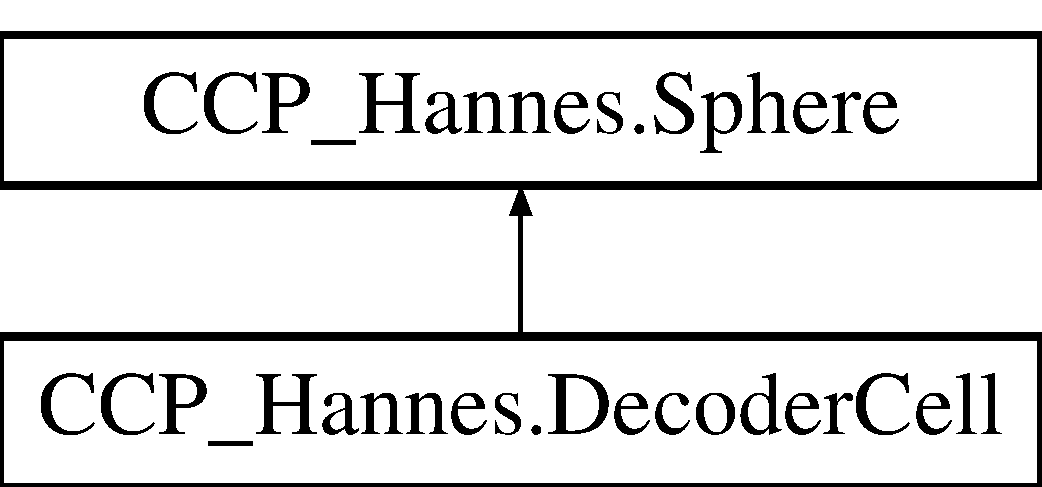
\includegraphics[height=2.000000cm]{class_c_c_p___hannes_1_1_decoder_cell}
\end{center}
\end{figure}
\subsection*{Public Member Functions}
\begin{DoxyCompactItemize}
\item 
\mbox{\Hypertarget{class_c_c_p___hannes_1_1_decoder_cell_a3b78453be5d5b389de2f141ad0151feb}\label{class_c_c_p___hannes_1_1_decoder_cell_a3b78453be5d5b389de2f141ad0151feb}} 
def {\bfseries \+\_\+\+\_\+init\+\_\+\+\_\+} (self, args)
\item 
def \mbox{\hyperlink{class_c_c_p___hannes_1_1_decoder_cell_afd9c75a3e3a0b21822db336db465df33}{express\+Lectins}} (self, lectin\+\_\+list, density\+\_\+percentage)
\begin{DoxyCompactList}\small\item\em Method to attach \mbox{\hyperlink{class_c_c_p___hannes_1_1_lectin}{Lectin}} objects to \mbox{\hyperlink{class_c_c_p___hannes_1_1_decoder_cell}{Decoder\+Cell}} objects. \end{DoxyCompactList}\end{DoxyCompactItemize}
\subsection*{Public Attributes}
\begin{DoxyCompactItemize}
\item 
\mbox{\Hypertarget{class_c_c_p___hannes_1_1_decoder_cell_afcf4b1d70245a88a187c0409e9697a43}\label{class_c_c_p___hannes_1_1_decoder_cell_afcf4b1d70245a88a187c0409e9697a43}} 
{\bfseries lectin\+\_\+density}
\item 
\mbox{\Hypertarget{class_c_c_p___hannes_1_1_decoder_cell_a156ae46d12ffe483195b5b9497f19dc5}\label{class_c_c_p___hannes_1_1_decoder_cell_a156ae46d12ffe483195b5b9497f19dc5}} 
{\bfseries lectin}
\end{DoxyCompactItemize}


\subsection{Detailed Description}
\mbox{\hyperlink{class_c_c_p___hannes_1_1_decoder_cell}{Decoder\+Cell}} is a subclass of \mbox{\hyperlink{class_c_c_p___hannes_1_1_sphere}{Sphere}} and represents immune cells (such as T\+H\+P-\/1 cells) that express Lectins which bind to \mbox{\hyperlink{class_c_c_p___hannes_1_1_glycan}{Glycan}} structures and engage in immune response by secreting cytokines. 



\subsection{Member Function Documentation}
\mbox{\Hypertarget{class_c_c_p___hannes_1_1_decoder_cell_afd9c75a3e3a0b21822db336db465df33}\label{class_c_c_p___hannes_1_1_decoder_cell_afd9c75a3e3a0b21822db336db465df33}} 
\index{C\+C\+P\+\_\+\+Hannes\+::\+Decoder\+Cell@{C\+C\+P\+\_\+\+Hannes\+::\+Decoder\+Cell}!express\+Lectins@{express\+Lectins}}
\index{express\+Lectins@{express\+Lectins}!C\+C\+P\+\_\+\+Hannes\+::\+Decoder\+Cell@{C\+C\+P\+\_\+\+Hannes\+::\+Decoder\+Cell}}
\subsubsection{\texorpdfstring{express\+Lectins()}{expressLectins()}}
{\footnotesize\ttfamily def C\+C\+P\+\_\+\+Hannes.\+Decoder\+Cell.\+express\+Lectins (\begin{DoxyParamCaption}\item[{}]{self,  }\item[{}]{lectin\+\_\+list,  }\item[{}]{density\+\_\+percentage }\end{DoxyParamCaption})}



Method to attach \mbox{\hyperlink{class_c_c_p___hannes_1_1_lectin}{Lectin}} objects to \mbox{\hyperlink{class_c_c_p___hannes_1_1_decoder_cell}{Decoder\+Cell}} objects. 

Every \mbox{\hyperlink{class_c_c_p___hannes_1_1_decoder_cell}{Decoder\+Cell}} objects contains one type of \mbox{\hyperlink{class_c_c_p___hannes_1_1_lectin}{Lectin}} with a given density. Parameter lectins\+\_\+list is handed over to the constructor of \mbox{\hyperlink{class_c_c_p___hannes_1_1_lectin}{Lectin}}.


\begin{DoxyParams}[1]{Parameters}
\mbox{\tt in}  & {\em lectin\+\_\+list} & see documentation for class \mbox{\hyperlink{class_c_c_p___hannes_1_1_lectin}{Lectin}}. \\
\hline
\end{DoxyParams}


The documentation for this class was generated from the following file\+:\begin{DoxyCompactItemize}
\item 
C\+C\+P\+\_\+\+Hannes.\+py\end{DoxyCompactItemize}

\hypertarget{class_c_c_p___hannes_1_1_glycan}{}\section{C\+C\+P\+\_\+\+Hannes.\+Glycan Class Reference}
\label{class_c_c_p___hannes_1_1_glycan}\index{C\+C\+P\+\_\+\+Hannes.\+Glycan@{C\+C\+P\+\_\+\+Hannes.\+Glycan}}


Objects of the class \mbox{\hyperlink{class_c_c_p___hannes_1_1_glycan}{Glycan}} are attached to objects of the class \mbox{\hyperlink{class_c_c_p___hannes_1_1_bead}{Bead}}.  


\subsection*{Public Member Functions}
\begin{DoxyCompactItemize}
\item 
\mbox{\Hypertarget{class_c_c_p___hannes_1_1_glycan_aafa365a1d9370f65fed0715a7d1f6a54}\label{class_c_c_p___hannes_1_1_glycan_aafa365a1d9370f65fed0715a7d1f6a54}} 
def {\bfseries \+\_\+\+\_\+init\+\_\+\+\_\+} (self, glycan\+\_\+names\+\_\+list, glycan\+\_\+types\+\_\+list)
\end{DoxyCompactItemize}
\subsection*{Public Attributes}
\begin{DoxyCompactItemize}
\item 
\mbox{\Hypertarget{class_c_c_p___hannes_1_1_glycan_a0c2be33e3ba5593a639bd47f24bcc1c4}\label{class_c_c_p___hannes_1_1_glycan_a0c2be33e3ba5593a639bd47f24bcc1c4}} 
{\bfseries name}
\item 
\mbox{\Hypertarget{class_c_c_p___hannes_1_1_glycan_a097d262d25212abbc886ff25d90f10cc}\label{class_c_c_p___hannes_1_1_glycan_a097d262d25212abbc886ff25d90f10cc}} 
{\bfseries type}
\end{DoxyCompactItemize}


\subsection{Detailed Description}
Objects of the class \mbox{\hyperlink{class_c_c_p___hannes_1_1_glycan}{Glycan}} are attached to objects of the class \mbox{\hyperlink{class_c_c_p___hannes_1_1_bead}{Bead}}. 

They represent glycan structures which are divided into different types.


\begin{DoxyParams}[1]{Parameters}
\mbox{\tt in}  & {\em glycan\+\_\+names\+\_\+list} & List of Strings containing the \char`\"{}real\char`\"{} names of \mbox{\hyperlink{class_c_c_p___hannes_1_1_glycan}{Glycan}} structures to be added to the \mbox{\hyperlink{class_c_c_p___hannes_1_1_bead}{Bead}}. List may contain any number of members, including 0 \\
\hline
\mbox{\tt in}  & {\em glycan\+\_\+types\+\_\+list} & List of Strings containing the respective types of \mbox{\hyperlink{class_c_c_p___hannes_1_1_glycan}{Glycan}} structures. These types determine the outcome of the interaction between \mbox{\hyperlink{class_c_c_p___hannes_1_1_bead}{Bead}} and \mbox{\hyperlink{class_c_c_p___hannes_1_1_decoder_cell}{Decoder\+Cell}} as specified in the cytokine dictionary. If the this list does not contain the same number of member as glycan\+\_\+names\+\_\+list, the program terminates. \\
\hline
\end{DoxyParams}


The documentation for this class was generated from the following file\+:\begin{DoxyCompactItemize}
\item 
C\+C\+P\+\_\+\+Hannes.\+py\end{DoxyCompactItemize}

\hypertarget{class_c_c_p___hannes_1_1_lectin}{}\section{C\+C\+P\+\_\+\+Hannes.\+Lectin Class Reference}
\label{class_c_c_p___hannes_1_1_lectin}\index{C\+C\+P\+\_\+\+Hannes.\+Lectin@{C\+C\+P\+\_\+\+Hannes.\+Lectin}}


Objects of the class \mbox{\hyperlink{class_c_c_p___hannes_1_1_lectin}{Lectin}} are attached to objects of the class \mbox{\hyperlink{class_c_c_p___hannes_1_1_decoder_cell}{Decoder\+Cell}}.  


\subsection*{Public Member Functions}
\begin{DoxyCompactItemize}
\item 
\mbox{\Hypertarget{class_c_c_p___hannes_1_1_lectin_ad0b481fc5f873f2e601b5d087c0d97a4}\label{class_c_c_p___hannes_1_1_lectin_ad0b481fc5f873f2e601b5d087c0d97a4}} 
def {\bfseries \+\_\+\+\_\+init\+\_\+\+\_\+} (self, lectin\+\_\+list)
\end{DoxyCompactItemize}
\subsection*{Public Attributes}
\begin{DoxyCompactItemize}
\item 
\mbox{\Hypertarget{class_c_c_p___hannes_1_1_lectin_ac681f373d9d37dfb0e66def9db71757c}\label{class_c_c_p___hannes_1_1_lectin_ac681f373d9d37dfb0e66def9db71757c}} 
{\bfseries name}
\end{DoxyCompactItemize}


\subsection{Detailed Description}
Objects of the class \mbox{\hyperlink{class_c_c_p___hannes_1_1_lectin}{Lectin}} are attached to objects of the class \mbox{\hyperlink{class_c_c_p___hannes_1_1_decoder_cell}{Decoder\+Cell}}. 

They represent lectin receptors which recognize certain sets of glycans on other cells, beads, viruses a.\+s.\+o. If there are more than one kind of Lectins, the type of \mbox{\hyperlink{class_c_c_p___hannes_1_1_lectin}{Lectin}} is chosen randomly for every \mbox{\hyperlink{class_c_c_p___hannes_1_1_lectin}{Lectin}} instance.


\begin{DoxyParams}[1]{Parameters}
\mbox{\tt in}  & {\em lectin\+\_\+list} & List of Strings containing the names of \mbox{\hyperlink{class_c_c_p___hannes_1_1_lectin}{Lectin}} receptors to be added to the \mbox{\hyperlink{class_c_c_p___hannes_1_1_decoder_cell}{Decoder\+Cell}}. These names appear in the dictionary. List may contain any number of members, including 0. \\
\hline
\end{DoxyParams}


The documentation for this class was generated from the following file\+:\begin{DoxyCompactItemize}
\item 
C\+C\+P\+\_\+\+Hannes.\+py\end{DoxyCompactItemize}

\hypertarget{class_c_c_p___hannes_1_1_simulation}{}\section{C\+C\+P\+\_\+\+Hannes.\+Simulation Class Reference}
\label{class_c_c_p___hannes_1_1_simulation}\index{C\+C\+P\+\_\+\+Hannes.\+Simulation@{C\+C\+P\+\_\+\+Hannes.\+Simulation}}


The documentation for this class was generated from the following file\+:\begin{DoxyCompactItemize}
\item 
C\+C\+P\+\_\+\+Hannes.\+py\end{DoxyCompactItemize}

\hypertarget{class_c_c_p___hannes_1_1_sphere}{}\section{C\+C\+P\+\_\+\+Hannes.\+Sphere Class Reference}
\label{class_c_c_p___hannes_1_1_sphere}\index{C\+C\+P\+\_\+\+Hannes.\+Sphere@{C\+C\+P\+\_\+\+Hannes.\+Sphere}}


\mbox{\hyperlink{class_c_c_p___hannes_1_1_sphere}{Sphere}} serves as superclass for the two spherical objects indroduced below.  


Inheritance diagram for C\+C\+P\+\_\+\+Hannes.\+Sphere\+:\begin{figure}[H]
\begin{center}
\leavevmode
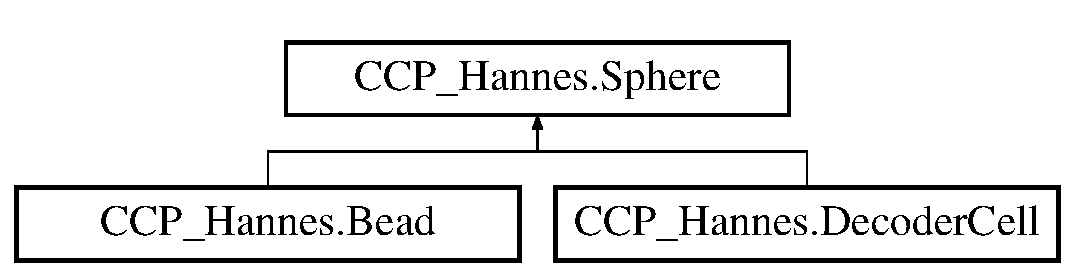
\includegraphics[height=2.000000cm]{class_c_c_p___hannes_1_1_sphere}
\end{center}
\end{figure}
\subsection*{Public Member Functions}
\begin{DoxyCompactItemize}
\item 
\mbox{\Hypertarget{class_c_c_p___hannes_1_1_sphere_a5e32ac3041f6e0463acc08642656bab7}\label{class_c_c_p___hannes_1_1_sphere_a5e32ac3041f6e0463acc08642656bab7}} 
def {\bfseries \+\_\+\+\_\+init\+\_\+\+\_\+} (self, I\+D\+\_\+string)
\end{DoxyCompactItemize}
\subsection*{Public Attributes}
\begin{DoxyCompactItemize}
\item 
\mbox{\Hypertarget{class_c_c_p___hannes_1_1_sphere_ac8db37d29aa6499edd50cc1e6378af51}\label{class_c_c_p___hannes_1_1_sphere_ac8db37d29aa6499edd50cc1e6378af51}} 
{\bfseries ID}
\item 
\mbox{\Hypertarget{class_c_c_p___hannes_1_1_sphere_a66c9c8500df0ede2af4705f993387733}\label{class_c_c_p___hannes_1_1_sphere_a66c9c8500df0ede2af4705f993387733}} 
{\bfseries coordinates}
\end{DoxyCompactItemize}


\subsection{Detailed Description}
\mbox{\hyperlink{class_c_c_p___hannes_1_1_sphere}{Sphere}} serves as superclass for the two spherical objects indroduced below. 


\begin{DoxyParams}[1]{Parameters}
\mbox{\tt in}  & {\em ID} & Identifier \\
\hline
 & {\em coordinates} & Empty. Will be filled when added to \mbox{\hyperlink{class_c_c_p___hannes_1_1_well}{Well}}. \\
\hline
\end{DoxyParams}


The documentation for this class was generated from the following file\+:\begin{DoxyCompactItemize}
\item 
C\+C\+P\+\_\+\+Hannes.\+py\end{DoxyCompactItemize}

\hypertarget{class_c_c_p___hannes_1_1_well}{}\section{C\+C\+P\+\_\+\+Hannes.\+Well Class Reference}
\label{class_c_c_p___hannes_1_1_well}\index{C\+C\+P\+\_\+\+Hannes.\+Well@{C\+C\+P\+\_\+\+Hannes.\+Well}}


The class \mbox{\hyperlink{class_c_c_p___hannes_1_1_well}{Well}} describes the sample, in which binding events take place.  


Inheritance diagram for C\+C\+P\+\_\+\+Hannes.\+Well\+:\begin{figure}[H]
\begin{center}
\leavevmode
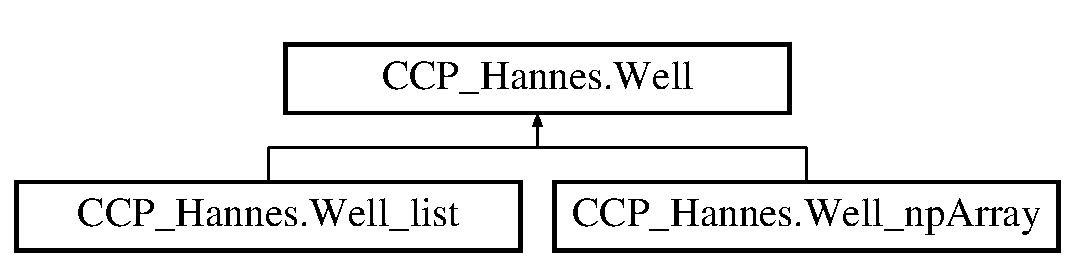
\includegraphics[height=2.000000cm]{class_c_c_p___hannes_1_1_well}
\end{center}
\end{figure}
\subsection*{Public Member Functions}
\begin{DoxyCompactItemize}
\item 
\mbox{\Hypertarget{class_c_c_p___hannes_1_1_well_a3149734033aad29ad56cca89fd2b8580}\label{class_c_c_p___hannes_1_1_well_a3149734033aad29ad56cca89fd2b8580}} 
def {\bfseries \+\_\+\+\_\+init\+\_\+\+\_\+} (self, x, y, z)
\item 
def \mbox{\hyperlink{class_c_c_p___hannes_1_1_well_ae595041538a36438fa0ff796a1e24d4c}{border\+Control}} (self, coordinates, dx, dy, dz)
\begin{DoxyCompactList}\small\item\em The method border\+Control ensures that objects\textquotesingle{} coordinates don\textquotesingle{}t exceed the \mbox{\hyperlink{class_c_c_p___hannes_1_1_well}{Well}}\textquotesingle{}s size. \end{DoxyCompactList}\end{DoxyCompactItemize}


\subsection{Detailed Description}
The class \mbox{\hyperlink{class_c_c_p___hannes_1_1_well}{Well}} describes the sample, in which binding events take place. 

It serves a a superclass for two subclasses of which one uses Num\+Py Arrays as a container for objects of the classes \mbox{\hyperlink{class_c_c_p___hannes_1_1_bead}{Bead}} and \mbox{\hyperlink{class_c_c_p___hannes_1_1_decoder_cell}{Decoder\+Cell}} while the other one uses built-\/in Python lists for this purpose.


\begin{DoxyParams}[1]{Parameters}
\mbox{\tt in}  & {\em x,y,z} & Size of the well. \\
\hline
\end{DoxyParams}


\subsection{Member Function Documentation}
\mbox{\Hypertarget{class_c_c_p___hannes_1_1_well_ae595041538a36438fa0ff796a1e24d4c}\label{class_c_c_p___hannes_1_1_well_ae595041538a36438fa0ff796a1e24d4c}} 
\index{C\+C\+P\+\_\+\+Hannes\+::\+Well@{C\+C\+P\+\_\+\+Hannes\+::\+Well}!border\+Control@{border\+Control}}
\index{border\+Control@{border\+Control}!C\+C\+P\+\_\+\+Hannes\+::\+Well@{C\+C\+P\+\_\+\+Hannes\+::\+Well}}
\subsubsection{\texorpdfstring{border\+Control()}{borderControl()}}
{\footnotesize\ttfamily def C\+C\+P\+\_\+\+Hannes.\+Well.\+border\+Control (\begin{DoxyParamCaption}\item[{}]{self,  }\item[{}]{coordinates,  }\item[{}]{dx,  }\item[{}]{dy,  }\item[{}]{dz }\end{DoxyParamCaption})}



The method border\+Control ensures that objects\textquotesingle{} coordinates don\textquotesingle{}t exceed the \mbox{\hyperlink{class_c_c_p___hannes_1_1_well}{Well}}\textquotesingle{}s size. 

If a step in {\ttfamily random\+Walk} would lead to a forbidden value, the sign of the respective step value will be reversed so the object \char`\"{}bounces
 back\char`\"{} from the \mbox{\hyperlink{class_c_c_p___hannes_1_1_well}{Well}}\textquotesingle{}s borders.


\begin{DoxyParams}[1]{Parameters}
\mbox{\tt in}  & {\em coordinates} & The object\textquotesingle{}s coordinates before the move. \\
\hline
\mbox{\tt in}  & {\em dx,dy,dz} & The randomly chosen next steps. \\
\hline
\mbox{\tt out}  & {\em dx,dy,dz} & The revised next steps. \\
\hline
\end{DoxyParams}


The documentation for this class was generated from the following file\+:\begin{DoxyCompactItemize}
\item 
C\+C\+P\+\_\+\+Hannes.\+py\end{DoxyCompactItemize}

\hypertarget{class_c_c_p___hannes_1_1_well__list}{}\section{C\+C\+P\+\_\+\+Hannes.\+Well\+\_\+list Class Reference}
\label{class_c_c_p___hannes_1_1_well__list}\index{C\+C\+P\+\_\+\+Hannes.\+Well\+\_\+list@{C\+C\+P\+\_\+\+Hannes.\+Well\+\_\+list}}


Subclass of \mbox{\hyperlink{class_c_c_p___hannes_1_1_well}{Well}} using built-\/in python lists as containers for objects of the classes \mbox{\hyperlink{class_c_c_p___hannes_1_1_bead}{Bead}} and \mbox{\hyperlink{class_c_c_p___hannes_1_1_decoder_cell}{Decoder\+Cell}}.  


Inheritance diagram for C\+C\+P\+\_\+\+Hannes.\+Well\+\_\+list\+:\begin{figure}[H]
\begin{center}
\leavevmode
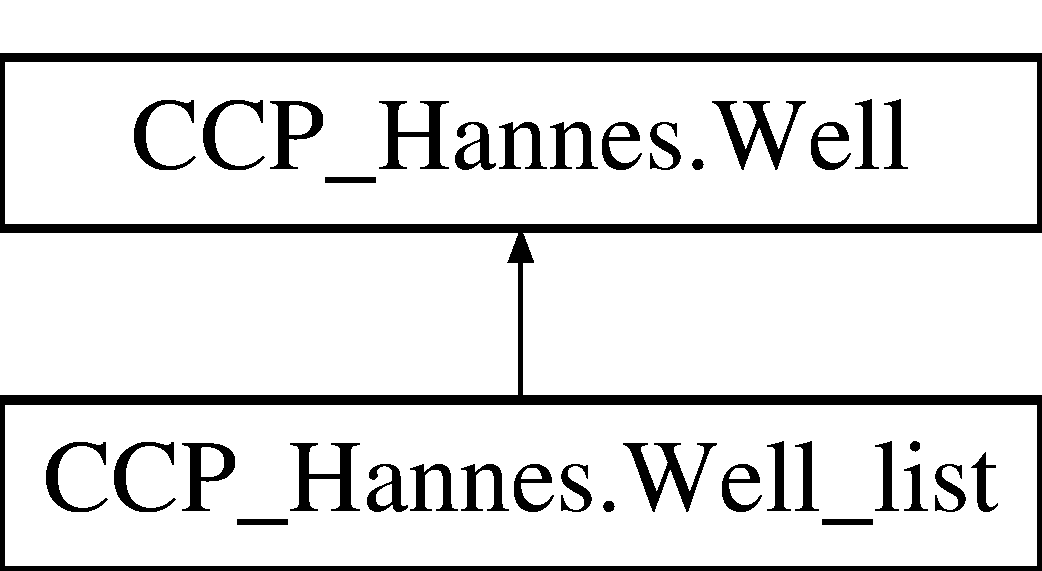
\includegraphics[height=2.000000cm]{class_c_c_p___hannes_1_1_well__list}
\end{center}
\end{figure}
\subsection*{Public Member Functions}
\begin{DoxyCompactItemize}
\item 
\mbox{\Hypertarget{class_c_c_p___hannes_1_1_well__list_a933f4992003c4596f01e5d6eb073dd98}\label{class_c_c_p___hannes_1_1_well__list_a933f4992003c4596f01e5d6eb073dd98}} 
def {\bfseries \+\_\+\+\_\+init\+\_\+\+\_\+} (self, x, y, z, n\+\_\+beads, n\+\_\+cells)
\item 
def \mbox{\hyperlink{class_c_c_p___hannes_1_1_well__list_ae4a512caba0dd7137b6ad4196cf72c1d}{add\+Bead}} (self, i, bead, glyan\+\_\+name\+\_\+string, glycan\+\_\+type\+\_\+string, density\+\_\+percentage)
\begin{DoxyCompactList}\small\item\em Method to add objects of class \mbox{\hyperlink{class_c_c_p___hannes_1_1_bead}{Bead}} to the bead list. \end{DoxyCompactList}\item 
\mbox{\Hypertarget{class_c_c_p___hannes_1_1_well__list_a5c1b28836c28ddea4d2cc808f4d1d266}\label{class_c_c_p___hannes_1_1_well__list_a5c1b28836c28ddea4d2cc808f4d1d266}} 
def {\bfseries add\+Decoder\+Cell} (self, i, decoder\+Cell, lectin\+\_\+name\+\_\+string, lectin\+\_\+type\+\_\+string)
\end{DoxyCompactItemize}
\subsection*{Public Attributes}
\begin{DoxyCompactItemize}
\item 
\mbox{\Hypertarget{class_c_c_p___hannes_1_1_well__list_a676c83197aea581b7a130d3e126bdca8}\label{class_c_c_p___hannes_1_1_well__list_a676c83197aea581b7a130d3e126bdca8}} 
{\bfseries size}
\item 
\mbox{\Hypertarget{class_c_c_p___hannes_1_1_well__list_a98e8a5739d0543e714fb0328d1ebeee9}\label{class_c_c_p___hannes_1_1_well__list_a98e8a5739d0543e714fb0328d1ebeee9}} 
{\bfseries beads}
\item 
\mbox{\Hypertarget{class_c_c_p___hannes_1_1_well__list_a2565b636a8563902152fbca021c0b84e}\label{class_c_c_p___hannes_1_1_well__list_a2565b636a8563902152fbca021c0b84e}} 
{\bfseries decoder\+Cells}
\end{DoxyCompactItemize}


\subsection{Detailed Description}
Subclass of \mbox{\hyperlink{class_c_c_p___hannes_1_1_well}{Well}} using built-\/in python lists as containers for objects of the classes \mbox{\hyperlink{class_c_c_p___hannes_1_1_bead}{Bead}} and \mbox{\hyperlink{class_c_c_p___hannes_1_1_decoder_cell}{Decoder\+Cell}}. 

\subsection{Member Function Documentation}
\mbox{\Hypertarget{class_c_c_p___hannes_1_1_well__list_ae4a512caba0dd7137b6ad4196cf72c1d}\label{class_c_c_p___hannes_1_1_well__list_ae4a512caba0dd7137b6ad4196cf72c1d}} 
\index{C\+C\+P\+\_\+\+Hannes\+::\+Well\+\_\+list@{C\+C\+P\+\_\+\+Hannes\+::\+Well\+\_\+list}!add\+Bead@{add\+Bead}}
\index{add\+Bead@{add\+Bead}!C\+C\+P\+\_\+\+Hannes\+::\+Well\+\_\+list@{C\+C\+P\+\_\+\+Hannes\+::\+Well\+\_\+list}}
\subsubsection{\texorpdfstring{add\+Bead()}{addBead()}}
{\footnotesize\ttfamily def C\+C\+P\+\_\+\+Hannes.\+Well\+\_\+list.\+add\+Bead (\begin{DoxyParamCaption}\item[{}]{self,  }\item[{}]{i,  }\item[{}]{bead,  }\item[{}]{glyan\+\_\+name\+\_\+string,  }\item[{}]{glycan\+\_\+type\+\_\+string,  }\item[{}]{density\+\_\+percentage }\end{DoxyParamCaption})}



Method to add objects of class \mbox{\hyperlink{class_c_c_p___hannes_1_1_bead}{Bead}} to the bead list. 

Coordinates of the \mbox{\hyperlink{class_c_c_p___hannes_1_1_bead}{Bead}} are randomly chosen between 0 and size of the \mbox{\hyperlink{class_c_c_p___hannes_1_1_well}{Well}} in the respective dimension.


\begin{DoxyParams}[1]{Parameters}
\mbox{\tt in}  & {\em i} & Not used here, but neccessary for convenient switching between container types. \\
\hline
\mbox{\tt in}  & {\em bead} & Object of class \mbox{\hyperlink{class_c_c_p___hannes_1_1_bead}{Bead}} to be added. \\
\hline
\mbox{\tt in}  & {\em } & \\
\hline
\end{DoxyParams}


The documentation for this class was generated from the following file\+:\begin{DoxyCompactItemize}
\item 
C\+C\+P\+\_\+\+Hannes.\+py\end{DoxyCompactItemize}

\hypertarget{class_c_c_p___hannes_1_1_well__np_array}{}\section{C\+C\+P\+\_\+\+Hannes.\+Well\+\_\+np\+Array Class Reference}
\label{class_c_c_p___hannes_1_1_well__np_array}\index{C\+C\+P\+\_\+\+Hannes.\+Well\+\_\+np\+Array@{C\+C\+P\+\_\+\+Hannes.\+Well\+\_\+np\+Array}}
Inheritance diagram for C\+C\+P\+\_\+\+Hannes.\+Well\+\_\+np\+Array\+:\begin{figure}[H]
\begin{center}
\leavevmode
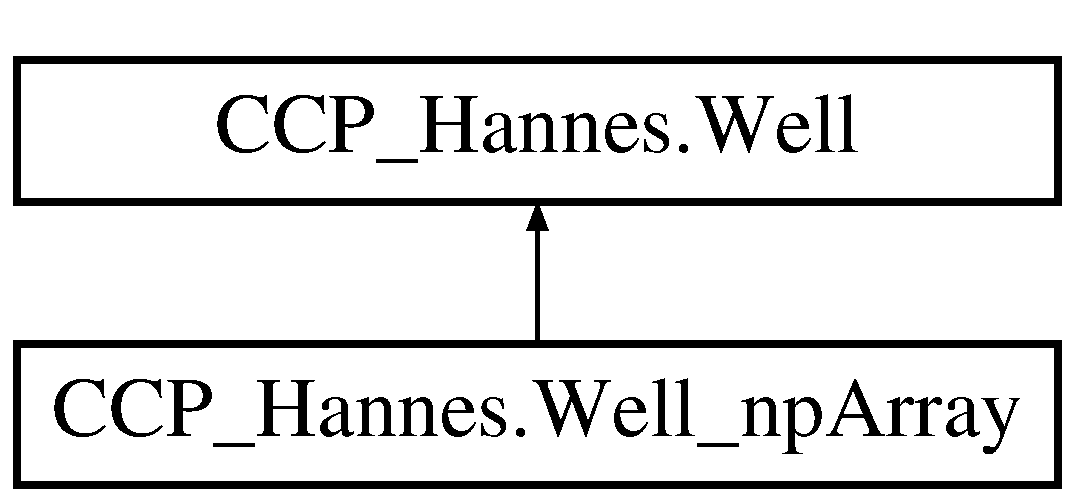
\includegraphics[height=2.000000cm]{class_c_c_p___hannes_1_1_well__np_array}
\end{center}
\end{figure}
\subsection*{Public Member Functions}
\begin{DoxyCompactItemize}
\item 
\mbox{\Hypertarget{class_c_c_p___hannes_1_1_well__np_array_ae9dcb8374add330e7be7bc24cf67b028}\label{class_c_c_p___hannes_1_1_well__np_array_ae9dcb8374add330e7be7bc24cf67b028}} 
def {\bfseries \+\_\+\+\_\+init\+\_\+\+\_\+} (self, x, y, z, n\+\_\+beads, n\+\_\+cells)
\item 
\mbox{\Hypertarget{class_c_c_p___hannes_1_1_well__np_array_a7284a17bcbf1187f6d35d8a0328ba39e}\label{class_c_c_p___hannes_1_1_well__np_array_a7284a17bcbf1187f6d35d8a0328ba39e}} 
def {\bfseries add\+Bead} (self, i, bead, glyan\+\_\+name\+\_\+string, glycan\+\_\+type\+\_\+string, density\+\_\+percentage)
\item 
\mbox{\Hypertarget{class_c_c_p___hannes_1_1_well__np_array_a9fb2c0fcfacb015b80ca23abe250e9ef}\label{class_c_c_p___hannes_1_1_well__np_array_a9fb2c0fcfacb015b80ca23abe250e9ef}} 
def {\bfseries add\+Decoder\+Cell} (self, i, decoder\+Cell, lectin\+\_\+name\+\_\+string, lectin\+\_\+type\+\_\+string)
\end{DoxyCompactItemize}
\subsection*{Public Attributes}
\begin{DoxyCompactItemize}
\item 
\mbox{\Hypertarget{class_c_c_p___hannes_1_1_well__np_array_ae2d7e1d206125d2565c35b97f57ab819}\label{class_c_c_p___hannes_1_1_well__np_array_ae2d7e1d206125d2565c35b97f57ab819}} 
{\bfseries size}
\item 
\mbox{\Hypertarget{class_c_c_p___hannes_1_1_well__np_array_acf36275f45a50a882d3f6f1edfb3e84d}\label{class_c_c_p___hannes_1_1_well__np_array_acf36275f45a50a882d3f6f1edfb3e84d}} 
{\bfseries beads}
\item 
\mbox{\Hypertarget{class_c_c_p___hannes_1_1_well__np_array_a8a744dba83859e9592fa5b61d799fc2b}\label{class_c_c_p___hannes_1_1_well__np_array_a8a744dba83859e9592fa5b61d799fc2b}} 
{\bfseries decoder\+Cells}
\end{DoxyCompactItemize}


The documentation for this class was generated from the following file\+:\begin{DoxyCompactItemize}
\item 
C\+C\+P\+\_\+\+Hannes.\+py\end{DoxyCompactItemize}

%--- End generated contents ---

% Index
\backmatter
\newpage
\phantomsection
\clearemptydoublepage
\addcontentsline{toc}{chapter}{Index}
\printindex

\end{document}
